\chapter[\'Etude en clinique]{\'Etude avec utilisation du test
  d'écoute en clinique psychiatrique}

Nous savons que la musicothérapie est de plus en plus intégrée dans
les milieux psychiatriques.
L'objectif ici est de vérifier l'hypothése évoquée et qui est celle de savoir s'il est possible d'estimer, après un travail 
musicothérapeutique, la transformation de l'écoute mesurée chez le
patient.
Les tests ont été faits en avril, mai, juin, juillet, septembre et octobre 2017.

\section{Cadre de travail}

 La Privatklinik
de Meiringen est  spécialisée en
addictologie dans le canton de Berne. Elle dispose d'une capacité de 195 lits, 33 médecins et
psychologues, secondés par 177 soignants qui assurent les soins du
patient.


\section{Organisation d'étude}

\subsection{Description des patients:}


-Moyenne d'âge:  entre 20 à 60 ans, masculin et féminin quasi égale.


-Pathologies:  burnout, dépendances, dépression.

-Temps de séjour: 3 à 6 semaines, voire plusieurs mois.
-Fréquence du traitement en musicothérapie: 1x par semaine pendant
50mn à 60mn.
-Le type de musicothérapie: habituelle dans ce contexte.
Ont été  exclu l'écoute avec casques et  musiques traitées chez Tomatis.
-Contexte de la clinique: contexte habituel d'une prise en
charge en clinique psychiatrique 
par les médecins et  les psychologues.
En plus, diverses thérapies sont proposées: physio--,ergo--,
art--,musico--,corporel--, zoo--  (chien/ cheval)  ainsi
que par les  ateliers de créativité sur le bois, la terre, la laine.  


\section{Design d'étude}

Mise en place:

Un groupe d'intervention A et un groupe de contrôle B ont été constitués.
La direction de la clinique ayant accepté l'étude, le personnel soignant et tout le
corpus des thérapies créatives ont  été
informés au préalable.

Les patients ont été avertis par un
court entretien individuel réalisé généralement par la musicothérapeute Regula Lehman  \footnote{Regula
  Lehmann, musicothérapeute  à 90\%  à la clinique de Meiringen.} et par  une
feuille explicative de notre démarche sur  l'évaluation de l'écoute et
sur
l'hypothèse de la transformation de cette écoute lors de leur 
séjour en thérapie. \emph{Information für Mitwirkende an der klinischen
  Studie\  ``Evaluierung des aktiven Hörvermögens" }.
Les patients étaient libres de participation. Ceux qui
l'ont fait, ont signé leur accord  officiellement à chaque fois  \emph{``Eine schriftliche Einbewilligung zum
Test"} avant de passer les deux types de tests dont nous nous sommes
occupés: Le questionnaire/test WHOQO-Bref et le test d'écoute.

 
 \subsection{Les patients}
 

\begin{itemize}
	\item 10 patients testés, groupe A en musicothérapie : un
          premier test avant leur prise en charge en musicothérapie;
          puis un 2\ieme\ test : après 4 semaines de
          clinique.
	\item 10 patients testés, groupe B de contrôle qui est un groupe sans musicothérapie,
	toujours dans le même contexte, c.à.dire la clinique, le suivi et les mêmes protocoles que l'autre groupe. Un premier test avant
	le début des autres thérapies puis un deuxième test, après 4 semaines. 
	
	Nous avons réalisé en tout 40 tests d'écoute. 
	
	Durée des tests : Chaque test d'écoute a une durée  moyenne de
        60 minutes par patient. Pour chacun, nous avons donc réalisé
        en tout deux heures de tests d'écoute avec un
        entretien(2x15').
        Le questionnaire WHOQOL (2x10mn)  a été remplis avant et après
        les séances en musicothérapie.
\end{itemize}

\section{Instruments de mesure: le WHOQO-Bref et le test d'écoute}
 

\subsection{Le WHOQO-Bref}

Nous avons utilisé et fait en parallèle le test WHOQO-Bref avant et
après pour avoir une variable supplémentaire pour confirmer en
parallèle supposée de l'action de la musicothérapie sur une éventuelle modification de l'écoute.  C'est une
version test de 1997 issue du Programme sur la santé mentale,
Organisation mondiale de la santé, Genève. Il y a 26 questions, que le
patient a rempli lui-même en présence du thérapeute, avant ou après le test
d'écoute. La durée pour les remplir a varié de 8 à 10 minutes en
moyenne.  Il a eu 26 tests WHOQO-Bref.

Il y a quatre domaines testés : physique, psychologique, relations sociales et environnement.
\begin{enumerate}
	\item  Le domaine de la perception physique comprend l' activité quotidienne// la dépendance et/ou l'assistance médicale// la fatigabilité, l'énergie//la mobilité// la douleur// le sommeil// la capacité de travail//
	
		 \item Le domaine psychologique :  image de soi, apparence// ressentis positifs et négatifs// estime de soi// spiritualité, croyances personnelles, religion// mémoire et concentration, apprentissage, pensée.
		
			\item Le domaine des relations sociales : relations personnelles// soutien social// vie sexuelle.
			
			\item Le domaine de l'environnement : l'environnement domestique et  physique (pollution, bruit, trafic, climat)// la situation financière//  la liberté, la sécurité physique et morale// l'accessibilité et qualité de la santé// les opportunités de détente, loisirs et d'acquisition d'informations// le transport// 
		\end{enumerate}
		
	


 \subsection{Le test d'écoute et les paramètres} 	
 
 \paragraph{Le test d'écoute avec l'appareil TSLT: conçu par Tomatis,
   cet appareil permet de traduire l'écoute par 
   un graphique l'écoute. La
   qualité de l'écoute est objectivée.} 
 Les paramètres: le seuil d'écoute, la fréquence, le volume sont des
 des paramètres 
 constituant d'un test d'écoute. Les courbes
 d'écoute aérienne et osseuse sont les résultats des
 réponses des patients. Leur réponse correspond à leur réaction à l'écoute d'une
 fréquence avec un volume précis.
 Le volume est augmenté individuellement et de manière progressive à
 chaque fréquence. Il sera arrêté lors du signal du patient. 
 
 
  \begin{enumerate}
 	\item les seuils d'écoute sont reconnaissables par des points au niveau de 
          chaque fréquence émise et selon le volume entendu par le patient. Les points reliés créent les courbes.
 	\item le son : son pur en 20 fréquences différentes.  
 	\item le volume: dB de $-20$ à 90; un carré sur le graphique représente une différence de \SI{5}{\dB} en
 		volume 
 	\item les fréquences: 20, de 125 à 8000 Hz. 
 	\item la courbe: est le résultat des points reliés des seuils
          d'écoute; ils 
          dessinent deux courbes caractéristiques, l'une aérienne et l'autre osseuse.
          L'observation des courbes d'écoute relevées vont permettre
          de les classer selon les paramètres d'harmonie ou
          d'équilibre, ceci 
 	en comparaison avec la courbe dite idéale : on parlera
        d'équilibre ou de
 	déséquilibre, d'harmonie ou de disharmonie.
        
      \item équilibre/déséquilibre graphique:
        -entre les deux oreilles
        -entre les deux courbes aérienne et osseuse mesurées pour
        l'oreille droite et l'oreille gauche.
        Des croisements, des pics ou des échancrures, un critère
        d'écart
        entre les deux courbes répertoriées vont être des
        données qui vont permettre de
        qualifier l'écoute d'harmonieuse ou de
        déséquilibrée. Ce pourrait ressembler à une lecture d'un
        électrocardiogramme.
        
 	\item La transformation de l'écoute: s'il y a une modification
          graphiques des courbes, elle 
          permettra d'évaluer la modification éventuelle de l'écoute et
          et de sa transformation.
          
\end{enumerate}
 
 	
        \subsection{Technique d'intervention musicothérapeutique:}
% ici tu peux crér a nouveau une liste. la numérotation est automatique.
% lis la doc.
\begin{enumerate}
        \item Premier test d'écoute et entretien
        \item Séances de musicothérapie, actives ou réceptives (1x par semaine)
        \item Deuxième test d'écoute et entretien
\end{enumerate}
        
 a) Les questions/réponses inhérents au 
 test d'écoute provoque le dialogue. Le patient est amené de façon
 détournée à se livrer et à évoquer des détails auxquels il
 n'aurait pas prêté attention. L'anamnèse prend donc ici un autre
 caractère puisqu'elle est complétée par le son et l'écoute.

 b)Les séances de musicothérapie se déroulent en
réceptif et actif. Elles n'ont pas été décortiquées et analysées
spécifiquement car ce n'était pas l'objectif de ce travail.		
        
 Le test d'écoute est en soi une forme d'intervention
 musicothérapeutique puisqu'il 
 a deux rôles intrinsèques:
% meme faute. APrès begin il faut n nom d'environnement: enumerate, itemize, center etc...

 la création d' une alliance thérapeutique et
     travail avec le son avec l'implication directe du
     patient dans le rôle de la 
     reconnaissance de sons
   
 Le test peut créer dès le premier entretien une alliance thérapeutique.
 D'autre part, il comporte un travail immédiat avec le son en impliquant le patient
 dans le rôle actif de leur reconnaissance. Il fait faire un travail de reconnaissance de sons dans
 l'espace (repérage de fréquences selon le volume). Le patient
 participe activement en fixant son attention sur les
 sons émis par l'appareil et transmis aux écouteurs en les repérant
  puis en y
 répondant. Cette implication directe conduit le patient à créer par lui-même et de manière
 inconsciente  
 son propre espace; ce  qui permettra par là même déjà d'entamer, pour certains dumoins, leur propre
 processus thérapeutique. (40% participe à la réussite d'une
                             % thérapie,(Sandra Lutz Hochreutener)
 
 	
 	
       

 	
 	\section{Un graphique}


        \begin{figure}
	\centering
	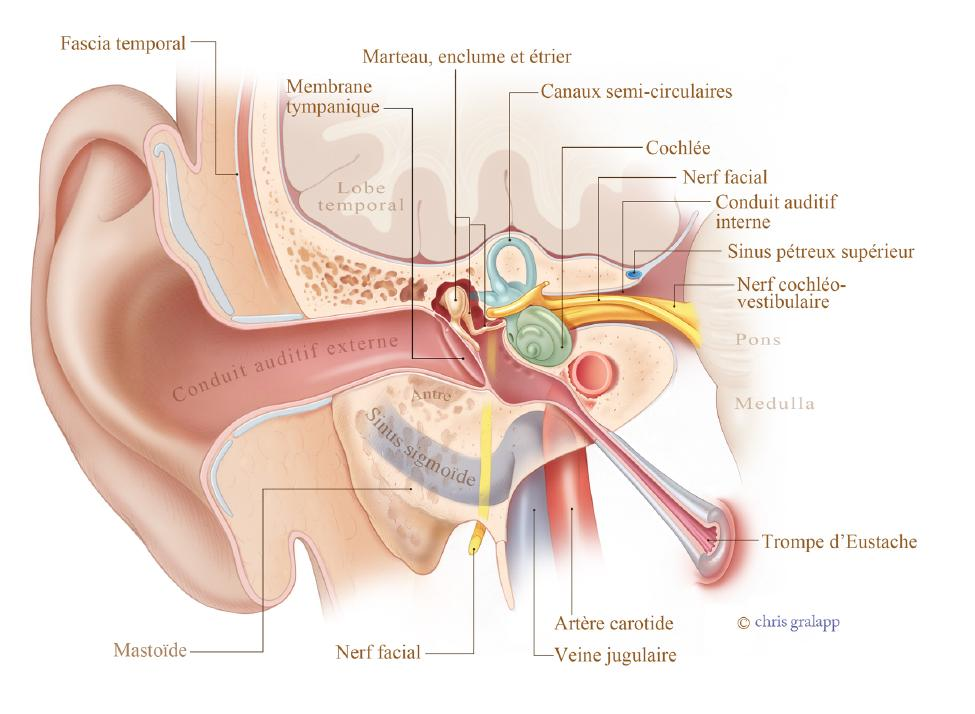
\includegraphics[width=1\linewidth]{images/20160624Berufsfeldgruppen.jpg}
	\caption[Anatomie oreille]{Anatomie de l'oreille}
	\label{valeriexxxx}
\end{figure}



                                      Patients souffrant de dépression, burnout
                                               en séjour dans la
                                               clinique
                                               \includegraphics[]{../../../Desktop/Groupe intervention,contrôle.png}


        
        Groupe de contrôle                                                    Groupe
                                                                                     d'intervention

1°test d'écoute avant thérapie, début de séjour           Idem+musicoth.

1°test WHOQO-Bref

                                                                                     Idem+musicoth.
2°Test en fin de thérapie, fin de séjour
2°Test WHOQO-Bref
 
 	
\section{Graphique d'écoute: 1°Test--2°test, considérations générales,
  comparaison}
	
 	
 	\subsection{Graphique du patient M avant musicoth.}
 	
 
 	
 	\begin{figure}[tbh]
 		\centering
 		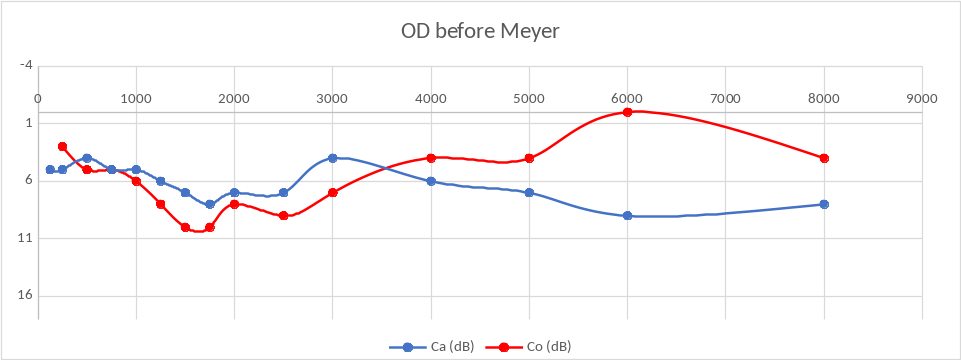
\includegraphics[width=0.7\linewidth]{images/clinique/od_before_meyer.png}
 		\caption{OD Avant Meyer}
 		\label{fig:odbeforemeyer}
 	\end{figure}
 	
 	\lipsum[1]
 	
 	
 	
 	
 	\begin{figure}
 		\centering
 		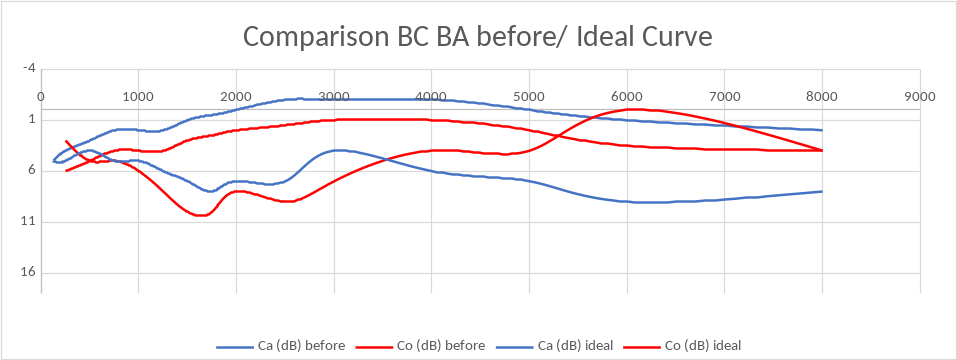
\includegraphics[width=0.7\linewidth]{images/clinique/comparison_bc_ba_before_vs_ideal_curve_meyer.png}
 		\caption[Avant vs courbe idéale]{Comparaison avant vs courbe idéale}
 		\label{fig:comparisonbcbabeforevsidealcurvemeyer}
 	\end{figure}
 	
 	
 	\subsection{Graphique du patient M après la musicoth.}
 	\lipsum[1]
 	\begin{figure}[h]
 		\centering

 		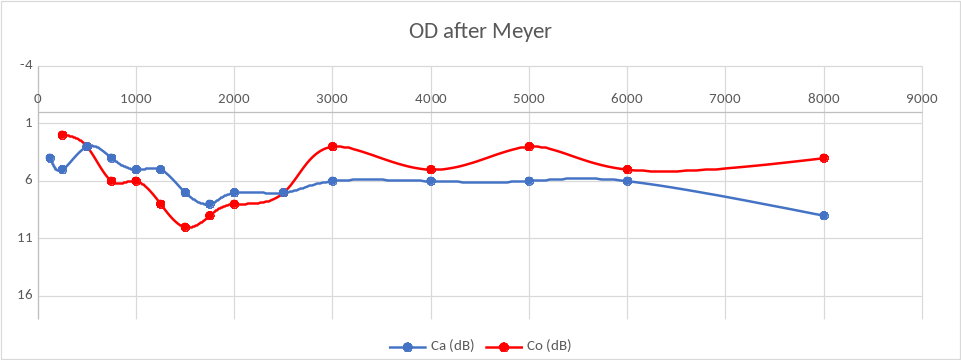
\includegraphics[width=0.7\linewidth]{images/clinique/od_after_meyer.png}
 		\caption{OD après vs courbe idéale}
 		\label{fig:odaftermeyer}
 	\end{figure}
 
 \lipsum[1]
 
 \begin{figure}[bh]
 	\centering
 	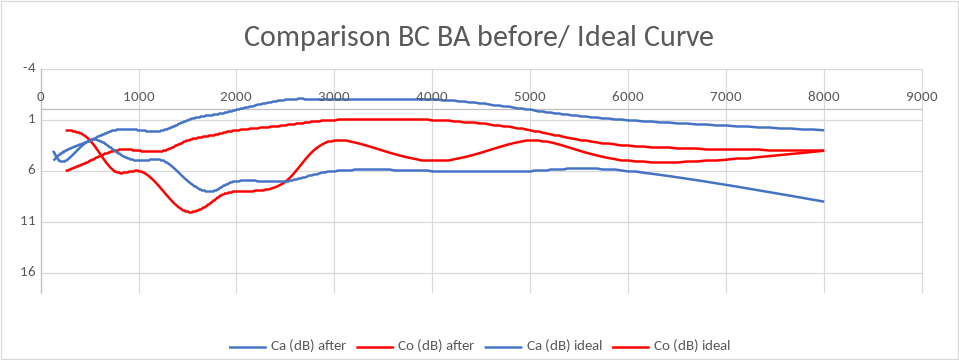
\includegraphics[width=0.7\linewidth]{images/clinique/comparison_bc_ba_after_vs_ideal_curve_meyer.png}
 	\caption{Comparaison après}
 	\label{fig:comparisonbcbaaftervsidealcurvemeyer}
 \end{figure}
 
 
\section{Les 3 zones avec leur résonance en musicothérapie et en
  psychologie}


	Informations croisées avec les informations récoltées par les 3 
          zones du test d'écoute:
          
Les paramètres utilisés en musicothérapie trouvent leur lien avec les
3 zones d'interprétation psychologique du test d'écoute.

-Le rythme, tempo, puls  =  Z.1: le physique, le corps, l'incorporéisation et
l'intégration du rythme,
la posture d'écoute.

-La voix, le timbre, la mélodie =  Z.2:  l'expression vocale, la communication,
l'émotionnel, la sensibilité, l'affect.

-La justesse= l'harmonie (consonance, dissonance) et l'improvisation = Z.3:  la créativité, l'interprétation, la
résonance, la musicalité, la motivation, le non-verbal (
l'intraduisible en mot), l'espace.


\subsection{La dépression, le burnout et leur expression musico--physico--psychologique:}

Les réactions physiologiques et psychologiques au stress et au burnout:
  Z.1: Le rythme cardiaque: un stress intense va modifier le rythme
  du corps en augmentant ses fréquences. La respiration deviendra
  rapide. Il va s'en suivre une modification des perceptions
  extérieures. Une sensibilité particulièrement accrue aux bruits et
  aux sons peut en découler et être vécue comme une
  atteinte physique et psychique insupportable.
  Le changement de posture et d'attitude corporelle sont
notables (affaissement) et la perte d'énergie physique considérable ( épuisement).

 Z.2: La qualité de la voix: changement de la qualité du timbre de la
 voix et de l'émission verbale.
  La voix se caractérise par son volume, son timbre, sa mélodie et son langage. 
 	
 	De manière très appropriées, nous pouvons faire ainsi le
        descriptif général de la voix d'un patient dépressif ou
        stressé avec: le volume, le timbre, la
        mélodie, le langage: 
 	\begin{enumerate}
 		\item le volume : basse intensité, faible dynamique
 		\item la mélodie : monotone, sans modulation
 		\item le timbre : mauvaise qualité due à une pertes des harmoniques
 		\item le langage : difficulté d'élocution, manque de fluidité
 	\end{enumerate}
        Il en découle une communication difficile avec l'entourage qui 
        conduit au retrait social et à l'enfermement sur soi.
        
Z.3: La confusion mentale, la démotivation, la perte d'énergie
psychique, la disharmonie intérieure/extérieure, le non-verbal.


\section{Graphique: Zones 1-2-3 du Test d'écoute // Musicothérapie}

.....



\section{Graphique:  WHOQO-Bref et Test d'écoute}

.........


\section{Résultats}

Schéma: ................................

\section{Réflexions}

\subsection{Le test}
Pourquoi un test?...
1)....







Le manque de temps a été le principal facteur  réducteur
de tests valables, les départs imprévus des patients, et/ou leur
absence momentanée (visite du psychologue, maladie, etc.). rajoutés au peu de temps de travail (10\%) ainsi qu'à la
contingence difficile due à la distance séparant Genève du lieu de travail (Meiringen)
: comment planifier un départ imprévu d'un patient !? il a fallu parfois
faire trois heures de route pour effectuer les tests finaux d'un ou deux
patients.
  
Par conséquent,  de nombreux tests sont restés 
incomplets et n'ont pu
être validés car ils ne remplissaient pas toutes les conditions requises.  En définitive, sur 40 tests d'écoute Tomatis et 26 tests
WHOQO-Bref, nous avons choisi de ressortir l'étude pour le groupe A de
5 patients effectifs en musicothérapie, tests complets, et le groupe
témoin B de 5 patients sur 9 effectifs, sans musicothérapie et tests
complets. 
 

  

  
  De manière très générale, les résultats obtenus ne
  sont pas significatifs.  La prise en charge en musicothérapie a eu lieu
  une fois par semaine pendant une heure, ce qui semble trop court pour observer un changement important. Nous pourrions émettre la supposition suivante :  est-ce qu'un un travail journalier, régulier aurait été indiqué pour des résultats plus rapidement visibles avec le test?
  Est-ce qu'une immersion plus intensive en musicothérapie transformerait l'écoute des patients ? 
   En comparaison avec des
  modifications importantes de courbes des tests observées généralement  lors d' une écoute
  régulière de deux heures par jour de musique pendant 15 jours --- en référence à l'entrainement des muscles de l'oreille chez Tomatis, qui, nous le rappelons, est une pédagogie de l'écoute --- il aurait été intéressant de pouvoir faire cette étude comparative dans cette clinique. Ainsi, nous aurions pu éventuellement mettre en avant  l'absolue nécessité de créer et d'instaurer systématiquement la musicothérapie dans de nombreuses institutions mais aussi  de la développer beaucoup plus intensément  si elle est déjà existante.
  Nous sommes clairement en présence d'une ébauche d'études, avec des pistes
  suggérées. 
  Cette étude est un mixe: quantitatif et qualitatif. Nous avons ainsi pris l'option de nous tenir à une
  observation, celle de la transformation de l'écoute.
  
  A fortiori, relevons le cas fort intéressant  d'une patiente du groupe B (sans
  musicothérapie) : lors du test, surprise d'apprendre en voyant son écoute que la musique pouvait la modifier, elle s'est mise à écouter assidûment du Mozart pendant son séjour en clinique, entre le 1° test et le second test.  Les résultats
  graphiques obtenus lors de sa sortie sont clairement significatifs
  et de plus sont en concordance avec le WHOQ-Bref!  
  Par conséquent, le test d'écoute a permis de lui faire prendre conscience d'une part que son écoute lui appartenait personnellement et d'autre part, qu'elle pouvait elle-même avoir un impact et jouer un rôle non seulement sur son écoute mais aussi sur sa propre  transformation.



   
   
   
   







\paragraph{Hypothèse}

Est-ce possible d'évaluer un travail musicothérapeutique au moyen
d'un test d'écoute?

Est-ce que le processus d'écoute en musicothérapie améliore la capacité
d'écoute ?

Est-ce que les test auditifs avant et après la musicothérapie permettent
de visualiser l'action de la musicothérapie?

\paragraph{Y-a-t-il une modification de l'écoute du patient après une prise
en charge en musicothérapie ?}

\paragraph{Est-ce que les résultats ($=$ un changement dans l'écoute) d'une prise
en charge musicothérapeutique peuvent être lisibles et visibles dans
un test d'écoute Tomatis ?}

Est-ce que ces résultats sont significatifs? 

\paragraph{Est-ce que l'écoute du patient s'est modifié ? si on a pu observer
une modification, dans quel sens va -t-elle ?}

Est-ce ce test valable ? est-ce que le contexte est suffisant pour
ressortir des résultats ?





